
% approximate-inference.tex

\documentclass[dvipdfmx,notheorems,t]{beamer}

\usepackage{docmute}

% settings.tex

\AtBeginDvi{\special{pdf:tounicode 90ms-RKSJ-UCS2}}

\AtBeginSection[]{\frame[t]{\frametitle{目次}
	\tableofcontents[currentsection,hideallsubsections]}}

\AtBeginSubsection[]{\frame[t]{\frametitle{目次}
	\tableofcontents[currentsection,currentsubsection,subsectionstyle=show/shaded/hide]}}

\usefonttheme{professionalfonts}
\usetheme{Madrid}

\setbeamercovered{transparent=30} 
% \setbeamertemplate{navigation symbols}{}
\setbeamertemplate{frametitle}[default][left]
\setbeamertemplate{frametitle continuation}{}
\setbeamertemplate{enumerate items}[square]
\setbeamertemplate{caption}[numbered]

\let\oldframe\frame
\renewcommand\frame[1][allowdisplaybreaks,allowframebreaks,t]{\oldframe[#1]}

\usepackage{bxdpx-beamer}
\usepackage{pxjahyper}
\usepackage{minijs}

\usepackage{amsmath}
\usepackage{amssymb}
\usepackage{amsthm}
\usepackage{bm}

\DeclareMathOperator*{\argmax}{arg\,max}
\DeclareMathOperator*{\argmin}{arg\,min}
\DeclareMathOperator{\Tr}{Tr}
\DeclareMathOperator{\KL}{KL}
\DeclareMathOperator{\diag}{diag}

\usepackage[T1]{fontenc}
\usepackage[utf8]{inputenc}

\setbeamertemplate{theorems}[numbered]
\theoremstyle{definition}
\newtheorem{theorem}{定理}
\newtheorem{definition}{定義}
\newtheorem{proposition}{命題}
\newtheorem{lemma}{補題}
\newtheorem{corollary}{系}
\newtheorem{conjecture}{予想}
\newtheorem*{remark}{Remark}
\renewcommand{\proofname}{}

\renewcommand{\figurename}{図}
\renewcommand{\tablename}{表}

\renewcommand{\kanjifamilydefault}{\gtdefault}


\begin{document}

\section{近似推論法}

\subsection{EMアルゴリズムが困難な場合}

\begin{frame}{EMアルゴリズムが困難な場合}

\begin{itemize}
	\item EMアルゴリズムで行う計算
	\begin{itemize}
		\item \alert{Eステップ}では、潜在変数の事後確率分布$p(\bm{Z} | \bm{X}, \bm{\theta}^\mathrm{old})$を計算
		\newline
		\item \alert{Mステップ}では、完全データ対数尤度$\ln p(\bm{X}, \bm{Z} | \bm{\theta})$の期待値を計算
		\begin{eqnarray}
			&& \mathcal{Q}(\bm{\theta}, \bm{\theta}^\mathrm{old}) = \sum_{\bm{Z}} p(\bm{Z} | \bm{X}, \bm{\theta}^\mathrm{old}) \ln p(\bm{X}, \bm{Z} | \bm{\theta}) \\
			&& \mathcal{Q}(\bm{\theta}, \bm{\theta}^\mathrm{old}) = \int_{\bm{Z}} p(\bm{Z} | \bm{X}, \bm{\theta}^\mathrm{old}) \ln p(\bm{X}, \bm{Z} | \bm{\theta}) d\bm{Z}
		\end{eqnarray}
		そして、$\mathcal{Q}(\bm{\theta}, \bm{\theta}^\mathrm{old})$を最大化するパラメータ$\bm{\theta}^\mathrm{new}$を求める
		\begin{equation}
			\bm{\theta}^\mathrm{new} = \argmax_{\bm{\theta}} \mathcal{Q}(\bm{\theta}, \bm{\theta}^\mathrm{old})
		\end{equation}
	\end{itemize}
\end{itemize}

\end{frame}

\begin{frame}{EMアルゴリズムが困難な場合}

\begin{itemize}
	\item EMアルゴリズムの困難さ
	\begin{itemize}
		\item 実際に扱うモデルでは、事後分布$p(\bm{Z} | \bm{X}, \bm{\theta}^\mathrm{old})$の計算や、事後分布に従った期待値$\mathcal{Q}(\bm{\theta}, \bm{\theta}^\mathrm{old})$の計算が、\alert{不可能であることが多い}
		\newline
		\item 隠れ変数の\alert{次元が高すぎる}
		\item 事後分布が\alert{複雑な形をしていて}、期待値を解析的に計算できない
		\newline
		\item \alert{連続変数}であれば、積分が閉形式の解を持たないかもしれない
		\item 空間の次元の問題や、被積分項の複雑さから、数値積分すら困難かもしれない
		\newline
		\item \alert{離散変数}であれば、期待値を計算するためには、\alert{潜在変数の可能な全ての組み合わせについての和を取る}必要がある
		\item 隠れ変数の次元が高くなると、組み合わせ数が指数的に増大する
		\item 計算量が大きすぎて、期待値の厳密な計算がもはや不可能
	\end{itemize}
\end{itemize}

\end{frame}

\begin{frame}{EMアルゴリズムが困難な場合}

\begin{itemize}
	\item 近似法
	\begin{itemize}
		\item EMアルゴリズムが困難であるとき、何らかの方法で\alert{近似}しなければならない
		\item 近似法は、\alert{確率的な近似}と、\alert{決定的な近似}の2つに分けられる
	\end{itemize} \
	
	\item 確率的な近似
	\begin{itemize}
		\item \alert{マルコフ連鎖モンテカルロ法}などの手法がある
		\item \alert{無限の計算資源があれば}、厳密な結果が得られる
		\item 実際には計算量が有限であるため、得られる解は近似解となる
	\end{itemize} \
	
	\item 決定的な近似
	\begin{itemize}
		\item 事後分布$p(\bm{Z} | \bm{X}, \bm{\theta})$を\alert{解析的に近似}する
		\item 事後分布に対して、\alert{何らかの仮定をおく}
		\item 例えば、\alert{単純な項の積として分解できる}、あるいは、(ガウス分布などの特別な)\alert{パラメトリックな分布である}といった仮定
	\end{itemize}
\end{itemize}

\end{frame}

\subsection{変分法}

\begin{frame}{変分推論}

\begin{itemize}
	\item ここで扱う近似法
	\begin{itemize}
		\item \alert{変分推論法}(Variational inference)あるいは\alert{変分ベイズ法}(Variational Bayes)について扱う
	\end{itemize} \
	
	\item \alert{変分推論}(Variational inference)
	\begin{itemize}
		\item 18世紀のオイラー、ラグランジュらによる\alert{変分法}(Calculus of variations)に起源をもつ
		\newline
		\item まずは、変分法について説明をしていく
	\end{itemize}
\end{itemize}

\end{frame}

\begin{frame}{変分法}

\begin{itemize}
	\item 関数と\alert{汎関数}の違い
	\begin{itemize}
		\item 通常の関数は、入力として値をとり、出力として関数の値を返す
		\item 通常の関数は、\alert{値から値への写像}である
		\newline
		\item 関数の導関数は、入力値を微小に変えたときに、出力の関数値がどの程度変わるかを表す
		\newline
		\item \alert{汎関数}(Functional)とは、入力として\alert{関数をとり}、出力として汎関数の\alert{値}を返す
		\item 汎関数は、\alert{関数から値への写像}である
		\newline
		\item \alert{汎関数微分}(Functional derivative)とは、\alert{入力関数が微小に変わったとき}に、出力の汎関数値がどの程度変わるかを表す
		\newline
		\item 汎関数の微分を、\alert{変分}という
	\end{itemize}
\end{itemize}

\end{frame}

\begin{frame}{変分法}

\begin{itemize}
	\item 汎関数の例
	\begin{itemize}
		\item エントロピー$H[p]$は、確率分布$p(x)$を入力として、以下の量を返す汎関数
		\begin{equation}
			H[p] = -\int p(x) \ln p(x) dx
		\end{equation}
	\end{itemize} \
	
	\item 汎関数の最適化
	\begin{itemize}
		\item 多くの問題は、\alert{汎関数の値を最適化する問題}として定式化できる
		\newline
		\item 汎関数の最適化とは、\alert{可能な全ての入力関数の中から}、汎関数の値を最大化、あるいは最小化するような\alert{関数を選び出す}ことである
		\newline
		\item 通常の最適化では、可能な全てのパラメータ(入力値)の中から、関数を最大化、あるいは最小化するような1つのパラメータを選び出す
		\newline
		\item 次は、いよいよ\alert{変分}の計算について説明する
	\end{itemize}
\end{itemize}

\end{frame}

\begin{frame}{変分法}

\begin{itemize}
	\item 変分法
	\begin{itemize}
		\item 通常の微分を使えば、ある関数$y(x)$を最大化(最小化)するような$x$の値が求められる
		\newline
		\item \alert{変分法}を使えば、汎関数$F[y]$を最大化(最小化)するような、関数$y(x)$が求められる
		\item 従って、可能な全ての関数$y(x)$の中から、$F[y]$を最大(最小)にするような関数が得られる
	\end{itemize} \
	
	\item 変分法によって解ける問題の例
	\begin{itemize}
		\item 2点を結ぶ最短経路は? (答えは直線)
		\item 最速降下曲線は? (答えはサイクロイド)
		\item \alert{エントロピーが最大}になるような確率分布は? (答えは\alert{ガウス分布})
	\end{itemize}
\end{itemize}

\end{frame}

\begin{frame}{変分法}

\begin{itemize}
	\item 通常の微分の表現
	\begin{itemize}
		\item 関数$y(x + \epsilon)$のテイラー展開は次のように記述できた
		\begin{eqnarray}
			y(x + \epsilon) &=& \sum_{n = 0}^\infty \frac{y^{(n)}(x)}{n!} \epsilon^n \\
			&=& y(x) + \frac{dy}{dx} \epsilon + \frac{1}{2!} \frac{d^2 y}{dx^2} \epsilon^2 + \frac{1}{3!} \frac{d^3 y}{dx^3} \epsilon^3 + \cdots \\
			&=& y(x) + \frac{dy}{dx} \epsilon + O(\epsilon^2)
		\end{eqnarray}
		
		\item これより微分$dy / dx$は、次のように求められる
		\item 変数$x$に微小な変化$\epsilon$を加え、このときの関数値$y(x + \epsilon)$を$\epsilon$の累乗形として表現する
		\item 最後に$\epsilon \to 0$の極限をとればよい
		\begin{equation}
			\frac{dy}{dx} = \lim_{\epsilon \to 0} \frac{y(x + \epsilon) - y(x)}{\epsilon}
		\end{equation}
	\end{itemize}
\end{itemize}

\end{frame}

\begin{frame}{変分法}

\begin{itemize}	
	\item 多変数関数$y(x_1, \ldots, x_D)$の偏微分の表現
	\begin{itemize}
		\item 多変数関数$y(x_1, \ldots, x_D)$のテイラー展開は次のように記述できた
		\begin{equation}
			\bm{D}^n = \left( \epsilon_1 \frac{\partial y}{\partial x_i} + \cdots + \epsilon_D \frac{\partial y}{\partial x_D} \right)^n
		\end{equation}
		上記のような演算子$\bm{D}$を考えれば
		\begin{eqnarray}
			&& y(x_1 + \epsilon_1, \ldots, x_D + \epsilon_D) \nonumber \\
			&=& \sum_{n = 0}^\infty \frac{1}{n!} (\bm{D}^n y)(x_1, \ldots, x_D) \\
			&=& y(x_1, \ldots, x_D) + \sum_{i = 1}^D \frac{\partial y}{\partial x_i} \epsilon_i + \frac{1}{2!} \sum_{i = 1}^D \sum_{j = 1}^D \frac{\partial^2 y}{\partial x_i x_j} \epsilon_i \epsilon_j + \nonumber \\
			&& \qquad \frac{1}{3!} \sum_{i = 1}^D \sum_{j = 1}^D \sum_{k = 1}^D \frac{\partial^3 y}{\partial x_i x_j x_k} \epsilon_i \epsilon_j \epsilon_k + \cdots
		\end{eqnarray}
		であるから
		\begin{eqnarray}
			&& y(x_1 + \epsilon_1, \ldots, x_D + \epsilon_D) \nonumber \\
			&=& y(x_1, \ldots, x_D) + \sum_{i = 1}^D \frac{\partial y}{\partial x_i} \epsilon_i + O(\epsilon^2)
		\end{eqnarray}
		
		\item これより偏微分$\partial y/\partial x_i$は、次のように求められる
		\begin{eqnarray}
			&& \frac{\partial y}{\partial x_i} = \lim_{\epsilon_i \to 0} \frac{1}{\epsilon_i} \left( y(x_1, \ldots, x_{i - 1}, x_i + \epsilon_i, x_{i + 1}, \ldots, x_D) - \right. \nonumber \\
			&& \qquad \left. y(x_1, \ldots, x_{i - 1}, x_i, x_{i + 1}, \ldots, x_D) \right)
		\end{eqnarray}
	\end{itemize}
\end{itemize}

\end{frame}

\begin{frame}{変分法}

\begin{itemize}
	\item 変分の表現
	\begin{itemize}
		\item 多少不正確だが、変分をどのように定義すればよいか考えてみる
		\newline
		\item ここで、各$x_i$に対する関数の値$z_i = y(x_i)$を個別の変数とみなして、次の関数$F(z_1, \ldots, z_D)$について考えてみよう
		\begin{eqnarray}
			&& F(z_1 + \epsilon \eta(x_1), \ldots, z_D + \epsilon \eta(x_D)) \nonumber \\
			&=& F(z_1, \ldots, z_D) + \sum_{i = 1}^D \frac{\partial F}{\partial z_i} \epsilon \eta(x_i) + O(\epsilon^2)
		\end{eqnarray}
		$z_i = y(x_i)$を代入してみると
		\begin{eqnarray}
			&& F(y(x_1) + \epsilon \eta(x_1), \ldots, y(x_D) + \epsilon \eta(x_D)) \nonumber \\
			&=& F(y(x_1), \ldots, y(x_D)) + \sum_{i = 1}^D \frac{\partial F}{\partial y(x_i)} \epsilon \eta(x_i) + O(\epsilon^2)
		\end{eqnarray}
		
		\item ここで$D \to \infty$の極限を取り、$x_1, \ldots, x_D$が、ある連続した区間$[a, b]$に含まれる、全ての実数を表すことにする
		\newline
		\item このとき$y(x_1), \ldots, y(x_D)$は、実数の区間$[a, b]$で定義される\alert{連続関数}$y(x)$として書けることが分かる
		\newline
		\item 同様に$y(x_1) + \epsilon \eta(x_1), \ldots, y(x_D) + \epsilon \eta(x_D)$は、実数の区間$[a, b]$で定義される\alert{連続関数}$y(x) + \epsilon \eta(x)$として、まとめることができる
		\newline
		\item 関数$\eta(x)$も、実数の区間$[a, b]$で定義される連続関数
		\item $\epsilon \eta(x)$は、$y(x)$に加わる\alert{摂動}として、考えることができる
		\newline
		\item 関数$F$は、関数$y(x)$や$y(x) + \epsilon \eta(x)$を入力として受け取る、\alert{汎関数}$F[y]$として解釈できるから、次のように書ける
		\begin{eqnarray}
			&& F(y(x_1) + \epsilon \eta(x_1), \ldots, y(x_D) + \epsilon \eta(x_D)) = \nonumber \\
			&& \qquad F[y(x) + \epsilon \eta(x)] \\
			&& F(y(x_1), \ldots, y(x_D)) = F[y(x)]
		\end{eqnarray}
		
		\item 以下の項は、入力を$y(x)$に摂動を加えて$y(x) + \epsilon \eta(x)$へと微小に変化させたときの、汎関数の($F[y(x)]$から$F[y(x) + \epsilon \eta(x)]$への)変化量を表している
		\begin{equation}
			\sum_{i = 1}^D \frac{\partial F}{\partial y(x_i)} \epsilon \eta(x_i)
		\end{equation}
		
		\item 点$x_i$における汎関数$F$の変化量を、$x_1, \ldots, x_D$の範囲について、即ち、実数の区間$[a, b]$について足し合わせていると解釈する
		\newline
		\item $D \to \infty$のとき、$x_1, \ldots, x_D$は区間$[a, b]$における全ての実数を表すから、総和を積分に置き換えられそうである
		\newline
		\item \color{red}汎関数の微分$\displaystyle \frac{\delta F}{\delta y(x)}$\normalcolor を使えば、次のように書ける
		\begin{eqnarray}
			&& \sum_{i = 1}^D \frac{\partial F}{\partial y(x_i)} \epsilon \eta(x_i) \nonumber \\
			&\Rightarrow& \int_a^b \frac{\delta F}{\delta y(x)} \epsilon \eta(x) dx = \epsilon \int_a^b \frac{\delta F}{\delta y(x)} \eta(x) dx
		\end{eqnarray}
		
		\item 結局、変分$\displaystyle \frac{\delta F}{\delta y(x)}$は次のように定義できる
		\begin{equation}
			\color{red}F[y(x) + \epsilon \eta(x)] = F[y(x)] + \epsilon \int_a^b \frac{\delta F}{\delta y(x)} \eta(x) dx + O(\epsilon^2)\normalcolor
		\end{equation}
		\item $F[y]$は、区間$[a, b]$で定義される関数$y$を受け取るとする
		\newline
		\item 変分$\delta F/\delta y$は、入力関数$y(x)$に、任意の微小な変化$\epsilon \eta(x)$を加えたときの、\color{red}汎関数$F[y]$の変化量\normalcolor として定義できる
		\item $\eta(x)$は$x$についての任意の関数
	\end{itemize}
\end{itemize}

\end{frame}

\begin{frame}{変分法}

\begin{figure}[h]
	\centering
	\includegraphics[clip,scale=0.75,trim=2cm 16.5cm 1cm 2cm,page=724]{../pattern-recognition-and-machine-learning.pdf}
	\caption{$y(x)$と$y(x) + \epsilon \eta(x)$の表現}
\end{figure}

\end{frame}

\begin{frame}{変分法}

\begin{itemize}
	\item 変分法の例
	\begin{itemize}
		\item 次の図\ref{fig:function-derivative-example}を使って、実際に変分を求めてみよう
		\newline
		\item 汎関数$F[y]$は、次のように定義されるとする
		\begin{equation}
			F[y] = \int_a^b y(x) dx
		\end{equation}
		
		\item 汎関数の値$F[y(x)], F[y(x) + \epsilon \eta(x)]$は次のようになる
		\begin{eqnarray}
			&& F[y(x)] = \int_a^b y(x) dx \\
			&& F[y(x) + \epsilon \eta(x)] = \int_a^b \left( y(x) + \epsilon \eta(x) \right) dx
		\end{eqnarray}
		
		\item $F[y(x) + \epsilon \eta(x)]$は次のように分解できる
		\begin{eqnarray}
			F[y(x) + \epsilon \eta(x)] &=& \int_a^b y(x) dx + \epsilon \int_a^b \eta(x) dx \\
			&=& F[y(x)] + \epsilon \int_a^b \eta(x) dx
		\end{eqnarray}
		
		\item ここで、変分の定義式は
		\begin{equation}
			F[y(x) + \epsilon \eta(x)] = F[y(x)] + \epsilon \int_a^b \frac{\delta F}{\delta y(x)} \eta(x) dx + O(\epsilon^2)
		\end{equation}
		であったので、上の2つの式を見比べれば、変分$\delta F/\delta y$は結局
		\begin{equation}
			\frac{\delta F}{\delta y(x)} = 1
		\end{equation}
		となることが分かる
	\end{itemize}
\end{itemize}

\end{frame}

\begin{frame}{変分法}

\begin{figure}[h]
	\centering
	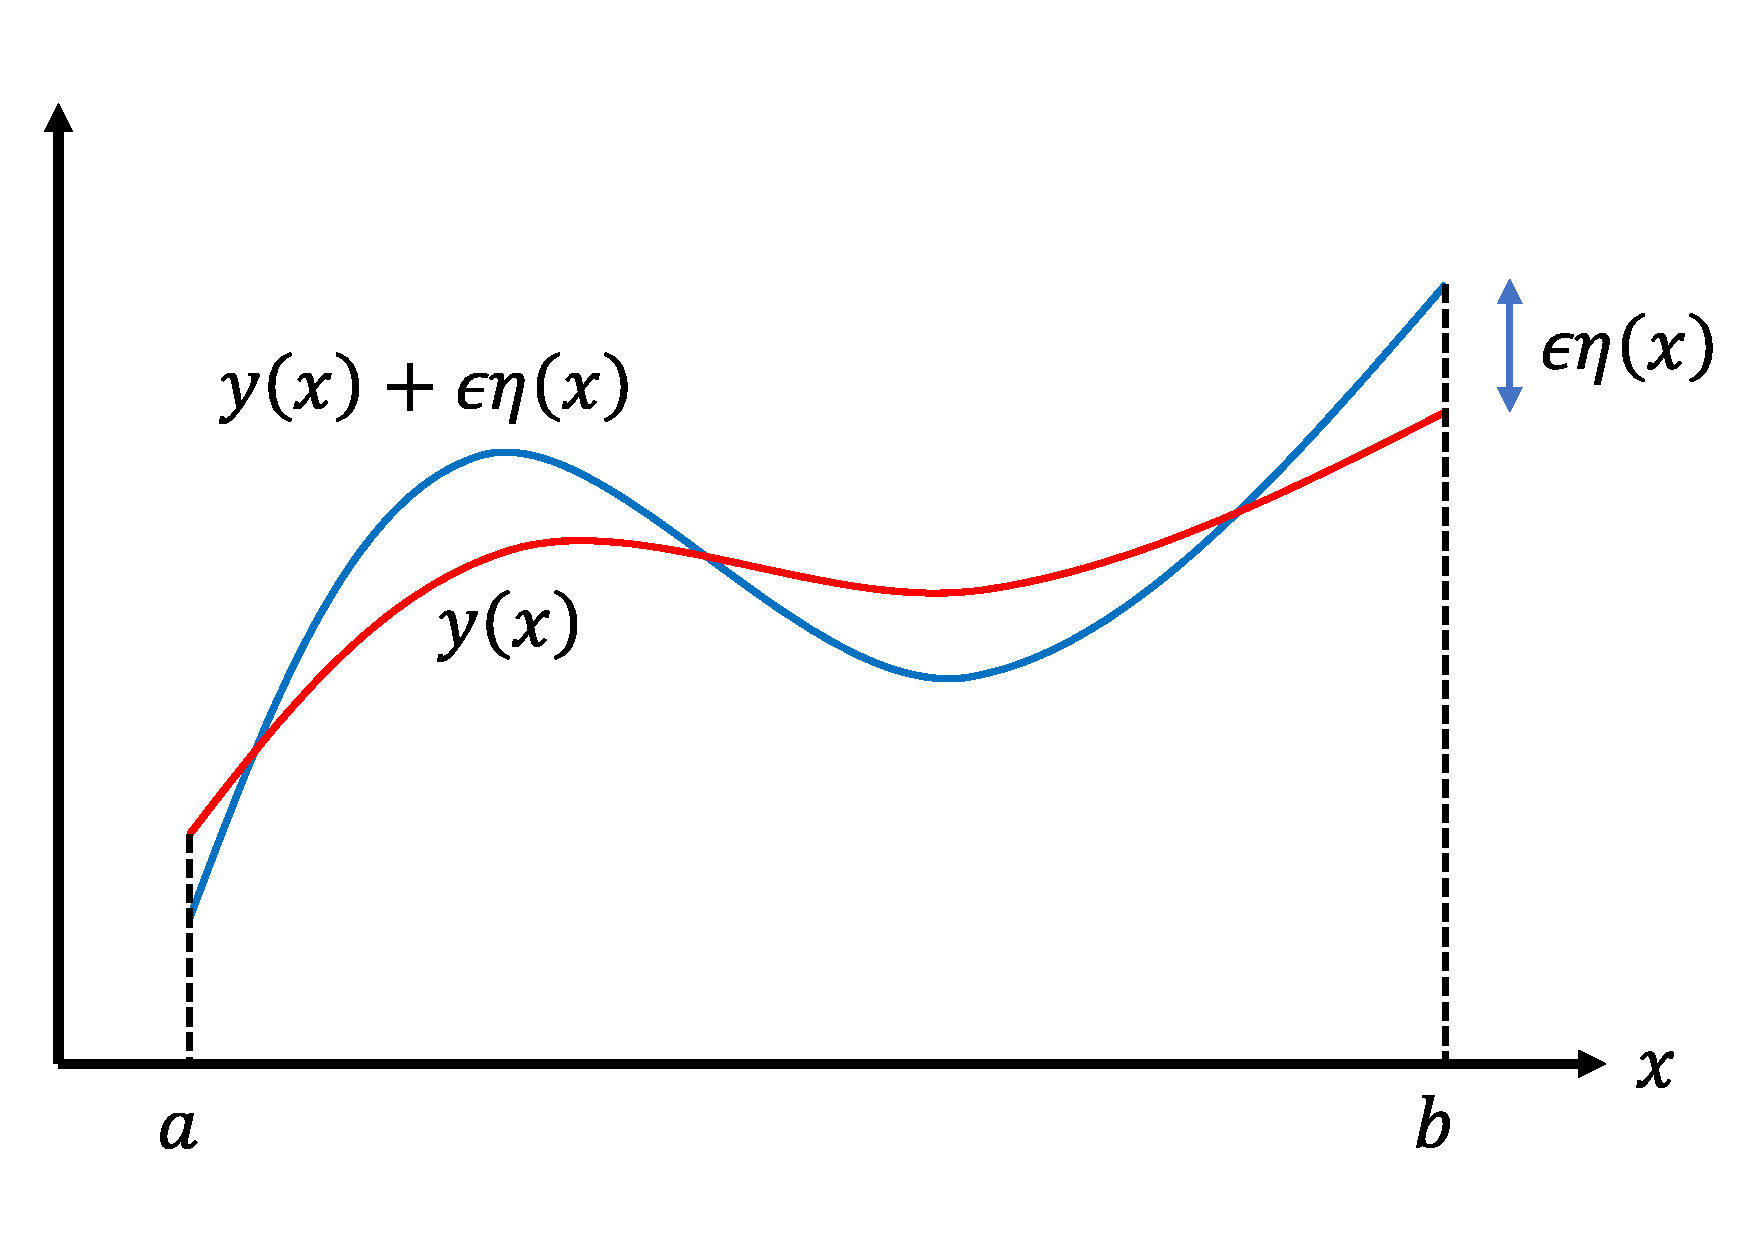
\includegraphics[scale=0.28]{functional-derivative.pdf}
	\caption{区間$[a, b]$で定義された関数$y(x)$の表現}
	\label{fig:function-derivative-example}
\end{figure}

\end{frame}

\begin{frame}{変分法}

\begin{itemize}
	\item 汎関数の最適化
	\begin{itemize}
		\item 汎関数$F[y]$が最大(最小)となるとき、\color{red}関数$y(x)$の微小な変化に対して、汎関数は変化しないはず\normalcolor
		\item 即ち、汎関数が最大(最小)となるとき、$F[y(x) + \epsilon \eta(x)] = F[y(x)]$が成り立つ
		\item 従って、変分の定義式から、以下が成り立つ
		\begin{equation}
			\int_a^b \frac{\delta F}{\delta y(x)} \eta(x) dx = 0
		\end{equation}
		
		\item 上式は任意の$\eta(x)$について成立しなければならない
		\item 従って、変分$\delta F/\delta y$は、任意の$x$について$0$とならなければならない
		\newline
		\item 汎関数$F[y]$が最大(最小)となるとき、\color{red}$\delta F/\delta y = 0$\normalcolor が成立することが分かった (\alert{通常の微分と同じ})
	\end{itemize}
\end{itemize}

\end{frame}

\begin{frame}{変分法}

\begin{itemize}
	\item 変分法の例
	\begin{itemize}
		\item 様々な汎関数について、変分を導出してみよう
		\item また、その汎関数が最大(最小)となるときに成り立つ条件を、導出してみよう
	\end{itemize}
\end{itemize}

\end{frame}

\begin{frame}{変分法}
	
\begin{itemize}
	\item 汎関数の例(1)
	\begin{itemize}
		\item $y(x)$とその微分$y'(x) = dy/dx$、そして$x$によって決まる関数\color{red}$G(y(x), y'(x), x)$\normalcolor があるとする
		\newline
		\item 汎関数$F[y]$を、$G(y(x), y'(x), x)$を区間$[a, b]$にわたって積分した結果を出力する関数として、次のように定める
		\begin{equation}
			F[y] = \int_a^b G(y(x), y'(x), x) dx
		\end{equation}
		
		\item 積分区間は無限であってもよいとする($a = -\infty, b = \infty$でもよい)
		\newline
		\item $y(x)$に摂動$\epsilon \eta(x)$を加えたときの、汎関数の値$F[y(x) + \epsilon \eta(x)]$を使って、変分$\delta F/\delta y$を調べてみる
		\begin{equation}
			F[y(x) + \epsilon \eta(x)] = \int_a^b G(y(x) + \epsilon \eta(x), y'(x) + \epsilon \eta'(x), x) dx
		\end{equation}
		ここで、被積分項のテーラー展開を考えれば
		\begin{eqnarray}
			&& G(y(x) + \epsilon \eta(x), y'(x) + \epsilon \eta'(x), x) \nonumber \\
			&=& G(y(x), y'(x), x) + \frac{\partial G}{\partial y} \epsilon \eta(x) + \nonumber \\
			&& \qquad \frac{\partial G}{\partial y'} \epsilon \eta'(x) + \frac{\partial G}{\partial x} \cdot 0 + O(\epsilon^2) \\
			&=& G(y(x), y'(x), x) + \epsilon \left( \frac{\partial G}{\partial y} \eta(x) + \frac{\partial G}{\partial y'} \eta'(x) \right) + O(\epsilon^2)
		\end{eqnarray}
		であるから
		\begin{eqnarray}
			&& F[y(x) + \epsilon \eta(x)] \nonumber \\
			&=& \int_a^b G(y(x) + \epsilon \eta(x), y'(x) + \epsilon \eta'(x), x) dx \nonumber \\
			&=& \int_a^b \bigg( G(y(x), y'(x), x) + \nonumber \\
			&& \qquad \left. \epsilon \left( \frac{\partial G}{\partial y} \eta(x) + \frac{\partial G}{\partial y'} \eta'(x) \right) + O(\epsilon^2) \right) dx \\
			&=& \int_a^b G(y(x), y'(x), x) dx + \nonumber \\
			&& \qquad \epsilon \int_a^b \left( \frac{\partial G}{\partial y} \eta(x) + \frac{\partial G}{\partial y'} \eta'(x) \right) dx + O(\epsilon^2) \\
			&=& F[y(x)] + \epsilon \int_a^b \left( \frac{\partial G}{\partial y} \eta(x) + \frac{\partial G}{\partial y'} \eta'(x) \right) dx + O(\epsilon^2)
		\end{eqnarray}
		ここで
		\begin{eqnarray}
			&& \int_a^b \left( \frac{\partial G}{\partial y} \eta(x) + \frac{\partial G}{\partial y'} \eta'(x) \right) dx \nonumber \\
			&=& \int_a^b \left( \frac{\partial G}{\partial y} \eta(x) \right) dx + \int_a^b \left( \frac{\partial G}{\partial y'} \eta'(x) \right) dx \\
			&=& \int_a^b \left( \frac{\partial G}{\partial y} \eta(x) \right) dx + \nonumber \\
			&& \qquad \left[ \frac{\partial G}{\partial y'} \eta(x) \right]_a^b - \int_a^b \frac{d}{dx} \left( \frac{\partial G}{\partial y'} \right) \eta(x) dx \\
			&=& \left[ \frac{\partial G}{\partial y'} \eta(x) \right]_a^b + \int_a^b \left( \frac{\partial G}{\partial y} - \frac{d}{dx} \left( \frac{\partial G}{\partial y'} \right) \right) \eta(x) dx
		\end{eqnarray}
		である
		\newline
		\item 途中の式変形では、部分積分を使っていることに注意
		\newline
		\item いま、積分区間の両端において、$y(x)$の値は固定されているとする
		\item これを\alert{固定端条件}という (図\ref{fig:function-derivative-example-2})
		\newline
		\item このとき、$\eta(a) = \eta(b) = 0$であるから、上式の最初の項が消えて
		\begin{eqnarray}
			&& \int_a^b \left( \frac{\partial G}{\partial y} \eta(x) + \frac{\partial G}{\partial y'} \eta'(x) \right) dx \nonumber \\
			&=& \left[ \frac{\partial G}{\partial y'} \eta(x) \right]_a^b + \int_a^b \left( \frac{\partial G}{\partial y} - \frac{d}{dx} \left( \frac{\partial G}{\partial y'} \right) \right) \eta(x) dx \\
			&=& \int_a^b \left( \frac{\partial G}{\partial y} - \frac{d}{dx} \left( \frac{\partial G}{\partial y'} \right) \right) \eta(x) dx
		\end{eqnarray}
		のようになる
		
		\item 従って、摂動を加えたときの汎関数の値$F[y(x) + \epsilon \eta(x)]$は
		\begin{eqnarray}
			&& F[y(x) + \epsilon \eta(x)] \nonumber \\
			&=& F[y(x)] + \epsilon \int_a^b \left( \frac{\partial G}{\partial y} - \frac{d}{dx} \left( \frac{\partial G}{\partial y'} \right) \right) \eta(x) dx + O(\epsilon^2)
		\end{eqnarray}
		となる
		\newline
		
		\item 上式を、変分の定義式と比べれば
		\begin{equation}
			F[y(x) + \epsilon \eta(x)] = F[y(x)] + \epsilon \int_a^b \frac{\delta F}{\delta y(x)} \eta(x) dx + O(\epsilon^2)
		\end{equation}
		変分$\delta F/\delta y$は次のように書ける
		\begin{equation}
			\color{red}\frac{\delta F}{\delta y(x)} = \frac{\partial G}{\partial y} - \frac{d}{dx} \left( \frac{\partial G}{\partial y'} \right)\normalcolor
		\end{equation}
		
		\item 汎関数$F[y]$が最大(最小)になるとき、変分$\delta F/\delta y$が$0$になる
		\item 従って、汎関数が最大(最小)になるとき、以下の方程式が成り立つ
		\begin{equation}
			\frac{\partial G}{\partial y} - \frac{d}{dx} \left( \frac{\partial G}{\partial y'} \right) = 0
		\end{equation}
		
		\item これを\alert{オイラー-ラグランジュ方程式}という
		\newline
		
		\item オイラー-ラグランジュ方程式は、次のような考え方で導出することもできる
		\newline
		\item $F[y]$が最大(最小)であれば、摂動$\epsilon \eta(x)$によって$y(x)$が少し変化しても、$F[y]$の値は変化しないはず
		\item 従って、$F[y]$が最大(最小)であるとき、\color{red}$F[y]$の$\epsilon$による微分は$0$になるはず\normalcolor
		
		\item これを数式で表現すると、次のようになる
		\begin{equation}
			\left. \frac{\partial F[y]}{\partial \epsilon} \right|_{\epsilon = 0} = 0
		\end{equation}
		左辺は通常の偏微分であり、これを計算すると
		\begin{eqnarray}
			&& \frac{\partial F[y]}{\partial \epsilon} \nonumber \\
			&=& \frac{\partial}{\partial \epsilon} \int_a^b G(y, y', x) dx \\
			&=& \int_a^b \frac{\partial}{\partial \epsilon} G(y, y', x) dx \\
			&=& \int_a^b \left( \frac{\partial G}{\partial y} \frac{\partial y}{\partial \epsilon} + \frac{\partial G}{\partial y'} \frac{\partial y'}{\partial \epsilon} + \frac{\partial G}{\partial x} \frac{\partial x}{\partial \epsilon} \right) dx \\
			&=& \int_a^b \left( \frac{\partial G}{\partial y} \eta(x) + \frac{\partial G}{\partial y'} \eta'(x) \right) dx \\
			&=& \left[ \frac{\partial G}{\partial y'} \eta(x) \right]_a^b + \int_a^b \left( \frac{\partial G}{\partial y} - \frac{d}{dx} \left( \frac{\partial G}{\partial y'} \right) \right) \eta(x) dx \\
			&& \qquad (\because \eta(a) = \eta(b) = 0) \nonumber \\
			&=& \int_a^b \left( \frac{\partial G}{\partial y} - \frac{d}{dx} \left( \frac{\partial G}{\partial y'} \right) \right) \eta(x) dx \\
			&=& 0 \nonumber
		\end{eqnarray}
		
		\item 上の式変形では、$y = y(x) + \epsilon \eta(x)$であるから
		\begin{eqnarray}
			&& \frac{\partial y}{\partial \epsilon} = \eta(x) \\
			&& \frac{\partial y'}{\partial \epsilon} = \frac{\partial}{\partial \epsilon} \left( \frac{\partial y}{\partial x} \right) = \frac{\partial}{\partial \epsilon} \left( y'(x) + \epsilon \eta'(x) \right) = \eta'(x) \\
			&& \frac{\partial x}{\partial \epsilon} = 0
		\end{eqnarray}
		が成立することを利用している
		\newline
		
		\item 任意の$\eta(x)$について、上式が恒等的に成り立つためには
		\begin{equation}
			\frac{\partial G}{\partial y} - \frac{d}{dx} \left( \frac{\partial G}{\partial y'} \right) = 0
		\end{equation}
		でなければならないことが分かり、先程と同様に、オイラー-ラグランジュ方程式を得る
	\end{itemize}
\end{itemize}

\end{frame}

\begin{frame}{変分法}

\begin{figure}[h]
	\centering
	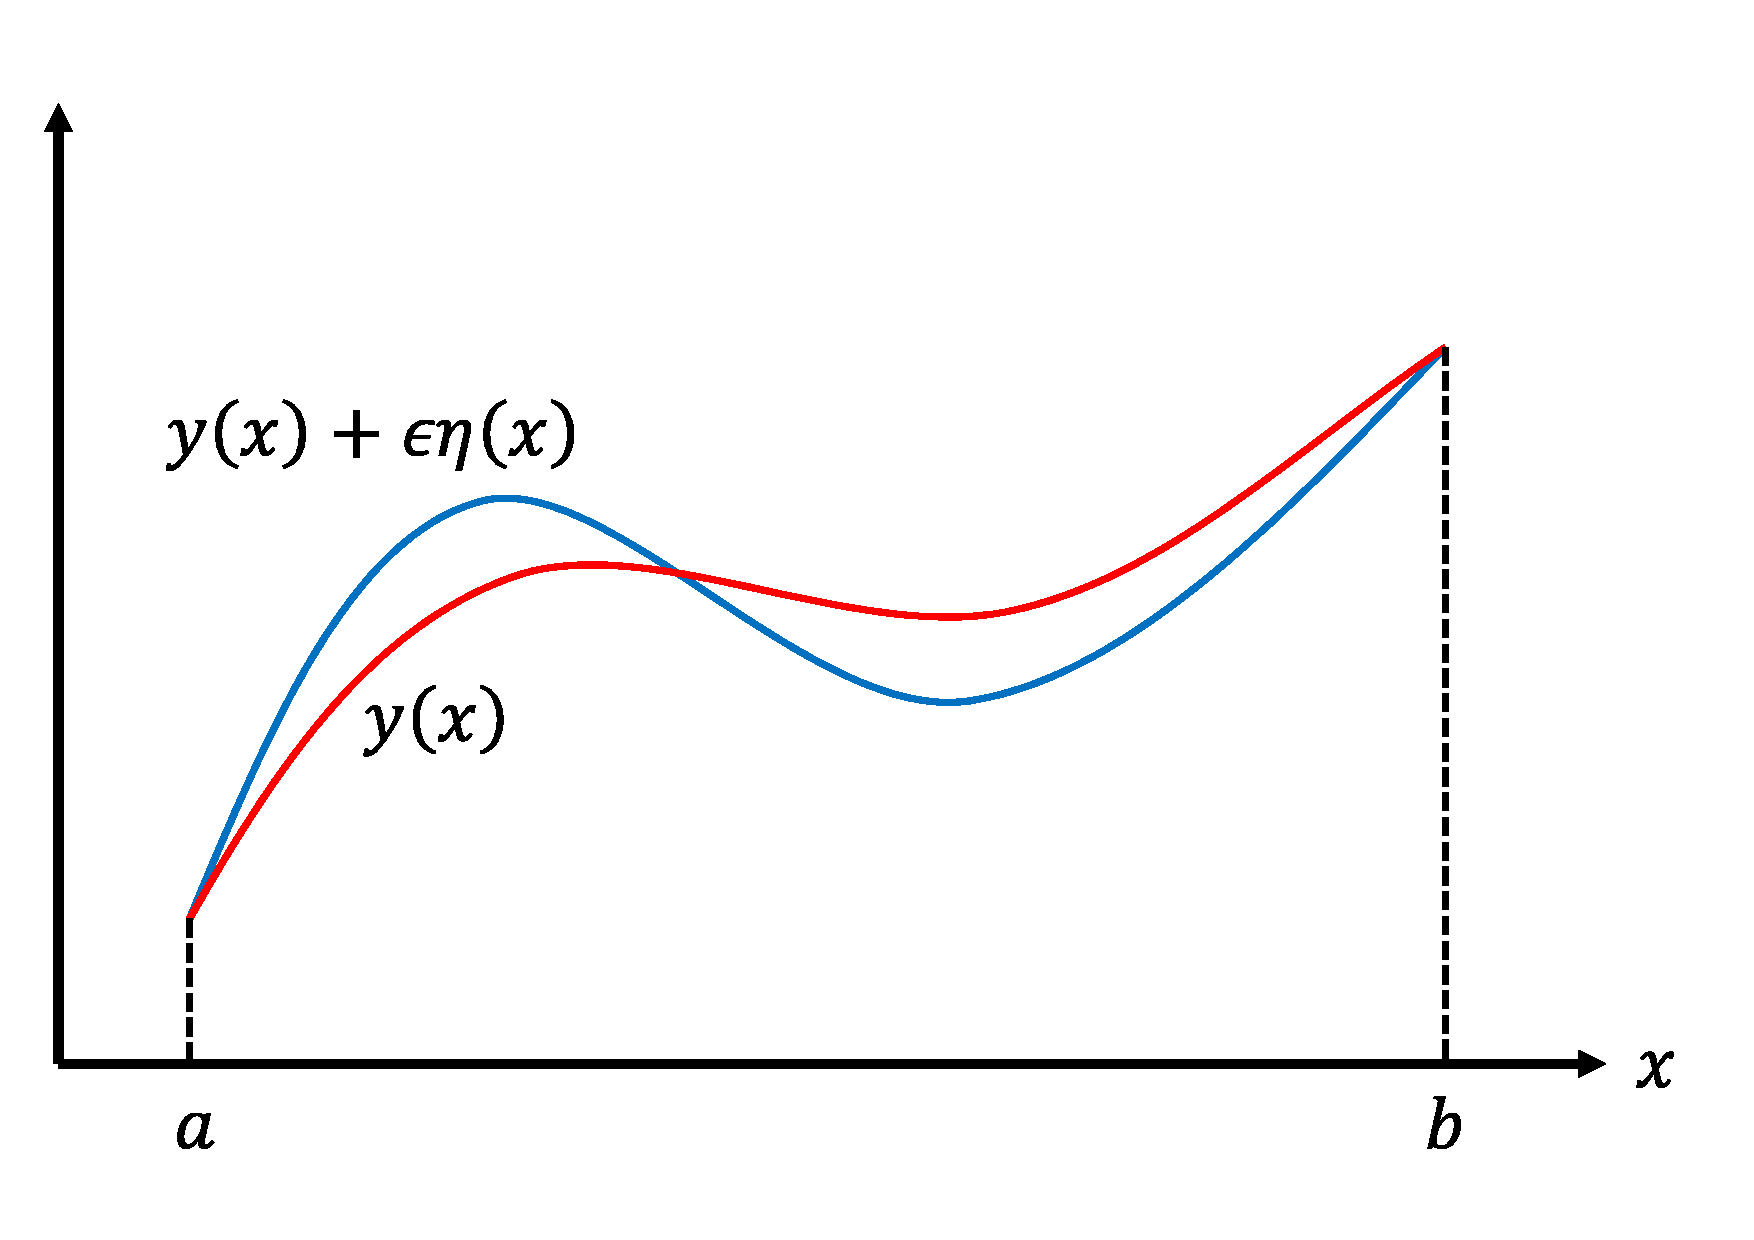
\includegraphics[scale=0.28]{functional-derivative-2.pdf}
	\caption{制約条件を含んでいる場合の表現}
	\label{fig:function-derivative-example-2}
\end{figure}

\end{frame}

\begin{frame}{変分法}

\begin{itemize}
	\item 汎関数の例(2)
	\begin{itemize}
		\item 上では$G(y(x), y'(x), x)$について考えて、変分を導出した
		\item $y(x)$と$x$のみによって決まり、$y'(x)$には依存しない関数\color{red}$G(y(x), x)$\normalcolor を考えよう
		\newline
		\item 汎関数$F[y]$は、先程と同様に以下で表されるとする
		\begin{equation}
			F[y] = \int_a^b G(y(x), x) dx
		\end{equation}
		
		\item このとき変分$\delta F/\delta y$を求めるのは、非常に簡単である
		\item 先程の式に、$\partial G/\partial y' = 0$を代入すれば直ちに得られる
		\begin{equation}
			\color{red}\frac{\delta F}{\delta y(x)} = \frac{\partial G}{\partial y}\normalcolor
		\end{equation}
		
		\item あるいは以下のように書ける
		\begin{equation}
			\color{red}\frac{\delta}{\delta y(x)} \int_a^b G(y(x), x) dx = \frac{\partial}{\partial y} G(y(x), x)\normalcolor
		\end{equation}
		
		\item $F[y]$が最大(最小)であるとき、以下のオイラー-ラグランジュ方程式が成り立つ
		\begin{equation}
			\frac{\partial G}{\partial y} = 0
		\end{equation}
	\end{itemize}
\end{itemize}

\end{frame}

\begin{frame}{変分法}

\begin{itemize}
	\item 汎関数の例(3)
	\begin{itemize}
		\item 今度は、$y'(x)$と$x$のみによって決まり、$y(x)$には依存しない関数\color{red}$G(y'(x), x)$\normalcolor を考えよう
		\newline
		\item この場合も変分$\delta F/\delta y$を求めるのは簡単である
		\item $G(y(x), y'(x), x)$の変分の式に、$\partial G/\partial y = 0$を代入すればよい
		\begin{equation}
			\color{red}\frac{\delta F}{\delta y(x)} = - \frac{d}{dx} \left( \frac{\partial G}{\partial y'} \right)
		\end{equation}
		
		\item オイラー-ラグランジュ方程式は次のようになる
		\begin{equation}
			- \frac{d}{dx} \left( \frac{\partial G}{\partial y'} \right) = 0
		\end{equation}
	\end{itemize}
\end{itemize}

\end{frame}

\begin{frame}{変分法}

\begin{itemize}
	\item 汎関数の例(4)
	\begin{itemize}
		\item $y(x)$と$y'(x)$によって決まる関数\color{red}$G(y(x), y'(x))$\normalcolor を考えよう
		\item このときのオイラー-ラグランジュ方程式を導出してみよう
		\newline
		\item $G(y(x), y'(x))$を$x$で微分すれば
		\begin{eqnarray}
			&& \frac{d}{dx} G(y, y') \nonumber \\
			&=& \frac{\partial}{\partial y} G(y, y') \frac{dy}{dx} + \frac{\partial}{\partial y'} G(y, y') \frac{dy'}{dx} \\
			&=& y' \frac{\partial}{\partial y} G(y, y') + \frac{\partial}{\partial y'} G(y, y') \frac{dy'}{dx}
		\end{eqnarray}
		となるから
		\begin{equation}
			y' \frac{\partial}{\partial y} G(y, y') = \frac{d}{dx} G(y, y') - \frac{\partial}{\partial y'} G(y, y') \frac{dy'}{dx}
		\end{equation}
		また、オイラー-ラグランジュ方程式の両辺に$y'$を掛けたものは
		\begin{equation}
			y' \frac{\partial}{\partial y} G(y, y') - y' \frac{d}{dx} \left( \frac{\partial}{\partial y'} G(y, y') \right) = 0
		\end{equation}
		これらを連立させて
		\begin{eqnarray}
			&& y' \frac{d}{dx} \left( \frac{\partial}{\partial y'} G(y, y') \right) = \frac{d}{dx} G(y, y') - \frac{\partial}{\partial y'} G(y, y') \frac{dy'}{dx} \\
			&& y' \frac{d}{dx} \left( \frac{\partial}{\partial y'} G(y, y') \right) + \frac{\partial}{\partial y'} G(y, y') \frac{dy'}{dx} = \frac{d}{dx} G(y, y') \\
			&& \frac{d}{dx} \left( y' \cdot \frac{\partial}{\partial y'} G(y, y') \right) = \frac{d}{dx} G(y, y') \\
			&& \int \left( \frac{d}{dx} \left( y' \cdot \frac{\partial}{\partial y'} G(y, y') \right) \right) dx = \nonumber \\
			&& \qquad \int \left( \frac{d}{dx} G(y, y') \right) dx + C \\
			&& G(y, y') = y' \cdot \frac{\partial}{\partial y'} G(y, y') + C
		\end{eqnarray}
		となるので、結局オイラー-ラグランジュ方程式は
		\begin{equation}
			G - y' \frac{\partial G}{\partial y'} = \mathrm{Const.}
		\end{equation}
		と書ける
	\end{itemize}
\end{itemize}

\end{frame}

\begin{frame}{変分法で解ける問題の例}

\begin{itemize}
	\item 変分法で解ける問題の例(1)
	\begin{itemize}
		\item 2点$P(0, 0)$、$Q(a, b)$を結ぶ最短経路は?
		\newline
		\item 2点を結ぶ経路$y = f(x)$($0 \le x \le a$)の長さ$l$は、次のようになる
		\begin{equation}
			l = \int_0^a \sqrt{1 + \left( \frac{dy}{dx} \right)^2} dx = \int_0^a \sqrt{1 + y'^2} dx
		\end{equation}
		
		\item 被積分項が$y'$のみの関数となっていることが分かる
		\item $G(y'(x), x)$の場合の公式を使えば、$l$の$y = f(x)$による変分が求まる
		\begin{eqnarray}
			\frac{\delta l}{\delta f(x)} &=& - \frac{d}{dx} \left( \frac{\partial}{\partial y'} \sqrt{1 + y'^2} \right) \\
			&=& - \frac{d}{dx} \left( \frac{1}{2} \frac{1}{\sqrt{1 + y'^2}} \frac{\partial}{\partial y'} \left( 1 + y'^2 \right) \right) \\
			&=& - \frac{d}{dx} \frac{y'}{\sqrt{1 + y'^2}}
		\end{eqnarray}
		
		\item $l$を最小化するような$y = f(x)$は、上式の変分を$0$と等置すれば
		\begin{eqnarray}
			&& - \frac{d}{dx} \frac{y'}{\sqrt{1 + y'^2}} = 0 \\
			&\therefore& \frac{y'}{\sqrt{1 + y'^2}} = \mathrm{Const.}
		\end{eqnarray}
		
		\item これは、\color{red}$y'$が定数である\normalcolor ことを意味している
		\item 従って、\color{red}$y = C_0 x + C_1$\normalcolor と書ける
		\newline
		\item 以上より、\color{red}2点間を結ぶ最短経路は直線\normalcolor である
		\newline
		\item $y = f(x)$の形について、\alert{具体的な仮定は特に置いていない}ことに注意
		\item 変分法では、\alert{関数そのものを最適化する}
		\item 従って、関数の具体的な形については、特に仮定する必要がない
	\end{itemize}
\end{itemize}

\end{frame}

\begin{frame}{変分法のまとめ}

\begin{itemize}
	\item 変分のまとめ
	\begin{itemize}
		\item これまでの計算で、次の変分が明らかとなった
		\begin{eqnarray}
			&& \frac{\delta}{\delta y(x)} \int G(y(x), y'(x), x) dx = \nonumber \\
			&& \qquad \frac{\partial}{\partial y} G(y(x), y'(x), x) - \frac{d}{dx} \left( \frac{\partial}{\partial y'} G(y(x), y'(x), x) \right) \\
			&& \frac{\delta}{\delta y(x)} \int G(y(x), x) dx = \frac{\partial}{\partial y} G(y(x), x) \\
			&& \frac{\delta}{\delta y(x)} \int G(y'(x), x) dx = - \frac{d}{dx} \left( \frac{\partial}{\partial y'} G(y'(x), x) \right)
		\end{eqnarray}
	\end{itemize}
\end{itemize}

\end{frame}

\begin{frame}{変分法のまとめ}

\begin{itemize}
	\item ここまでの話の流れ
	\begin{enumerate}
		\item 変分の定義や、変分の計算法について調査した
		\newline
		\item \alert{変分}(汎関数の微分)とは、入力関数が微小に変化したときの、出力値の変化量として定義される
		\newline
		\item 汎関数が特定の形で表せるとき、変分がどのようになるか計算した
		\item 汎関数が最大(最小)になるとき、\alert{オイラー-ラグランジュ方程式}が成立した
		\newline
		\item 変分法を用いて、2点間を結ぶ最短経路が\alert{直線}になることを確認した
	\end{enumerate} \
	
	\item これからの話の流れ
	\begin{itemize}
		\item 変分最適化を、どのように推論問題に適用するのかについて調べていく
	\end{itemize}
\end{itemize}

\end{frame}

\subsection{変分推論}

\begin{frame}{変分推論}

\begin{itemize}
	\item 変分推論が必要だった理由
	\begin{itemize}
		\item 潜在変数に関する事後分布$p(\bm{Z} | \bm{X}, \bm{\theta})$の計算は、困難であることが多い
		\item $p(\bm{Z} | \bm{X}, \bm{\theta})$の厳密な計算は諦める代わりに、\alert{別の確率分布で近似}したい
		\newline
		\item 別の確率分布で近似するとき、単純な項の積として表現できるといった、\alert{何らかの仮定を置く}
	\end{itemize} \
	
	\item 変分推論の目的
	\begin{itemize}
		\item 同時分布$p(\bm{X}, \bm{Z})$が求まっているときに、事後分布$p(\bm{Z} | \bm{X})$と、\alert{エビデンス}$p(\bm{X})$の近似を求める
	\end{itemize} \
	
	\item 注意点
	\begin{itemize}
		\item 観測変数と潜在変数をまとめて、$\bm{X}, \bm{Z}$とおく
		\item $p(\bm{X})$は、確率モデルからデータ$\bm{X}$が生起する確率である
		\item \alert{データからみたモデルの好み}と解釈できるから、$p(\bm{X})$を\alert{モデルエビデンス}という
	\end{itemize}
\end{itemize}

\end{frame}

\end{document}
